\documentclass[12pt, a4paper]{article}
%=========================== PACKAGES =============================%

\usepackage[utf8]{inputenc}
\DeclareUnicodeCharacter{00A0}{ }

\usepackage[hmargin=1.5cm,vmargin=1.5cm]{geometry}
\usepackage[brazil]{babel}

\usepackage{graphicx}
\usepackage{placeins}
\usepackage{subcaption}
\usepackage{float}

\usepackage{hhline}
\usepackage{courier}
 
\usepackage{amsmath}
\usepackage{bm}
\usepackage{amsfonts}

\usepackage{hyperref}

\usepackage{listings}
\renewcommand\lstlistingname{Programa}
\usepackage{color} %red, green, blue, yellow, cyan, magenta, black, white
\definecolor{mygreen}{RGB}{28,140,0} % color values Red, Green, Blue
\definecolor{mylilas}{RGB}{170,55,241} 
\lstset{language=Matlab,%
    %basicstyle=\color{red},
    basicstyle=\footnotesize\ttfamily,
    breaklines=true,%
    morekeywords={matlab2tikz},
    keywordstyle=\color{blue},%
    morekeywords=[2]{1}, keywordstyle=[2]{\color{black}},
    identifierstyle=\color{black},%
    stringstyle=\color{mylilas},
    commentstyle=\color{mygreen},%
    showstringspaces=false,%without this there will be a symbol in the places where there is a space
    numbers=left,%
    numberstyle={\tiny \color{black}},% size of the numbers
    numbersep=9pt, % this defines how far the numbers are from the text
    emph=[1]{for,end,break},emphstyle=[1]\color{red}, %some words to emphasise
    %emph=[2]{word1,word2}, emphstyle=[2]{style},    
    frame= single,
}

\usepackage{multirow}


\usepackage{steinmetz}
\usepackage{float}

%=========================== PACKAGES =============================%

\setcounter{section}{1}

\author{Gustavo Ciotto Pinton}

\begin{document}

\begin{titlepage}
\vspace*{.28\textheight}
\begin{center}
%
\begin{figure}[h]
    \centering
    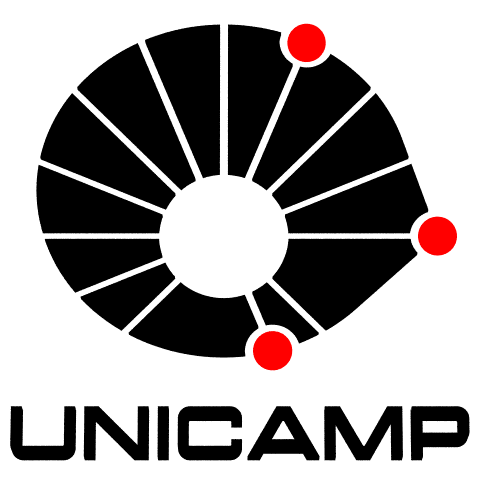
\includegraphics[scale=0.18]{image/LogoUnicamp}
\end{figure} 
%
\vspace*{10pt}
%\text{ }\\[7 cm]
\textbf{\LARGE Exercício de Fixação de Conceitos 2} \\ \vspace{12pt}
\textbf{\large EA072 - Inteligência Artificial em Aplicações Industriais}
\vspace*{72pt}

Gustavo \textbf{CIOTTO PINTON} - \textbf{RA 117136}
 

Campinas, \today

\end{center}
\end{titlepage}

\newpage
%  
% {\large 
%     \centerline{\textbf{Exercício de Fixação de Conceitos 1}}
%     \centerline{Gustavo Ciotto Pinton - 117136}
%     \centerline{EA072 - Inteligência Artificial em Aplicações Industriais}
% }

\section{Aproximação de funções multidimensionais}

\subsection {Mapeamento y = f(x)}

A função escolhida para o mapeamento \(\mathbb{R}^1 \rightarrow \mathbb{R}^1\)
está representada logo abaixo. Foi definido que o intervalo de \(x\) é
\([-2\pi,2\pi]\) e que este intervalo seria discretizado a cada 0.01, a fim de
possuirmos uma quantidade grande de amostras, isto é, 1257.

\begin{equation}
y = \exp(\sin x + \cos x) + \left|x\right|
\label{eq:map1}
\end{equation}

Sem a presença de ruídos, este mapeamento produz a imagem
\ref{fig:map1_s_ruido}. A imagem \ref{fig:map1_c_ruido}, por sua vez, apresenta
o resultado da soma da função com um ruído de distribuição normal de média nula
e variância 0.64. É possível verificar que a adição do ruído prejudica
fortemente a identificação do formato inicial do mapeamento. 

\FloatBarrier
			    
	\begin{figure}[h!]
	
	\centering
	
		\begin{subfigure}{.5\textwidth} 
		  \centering
		  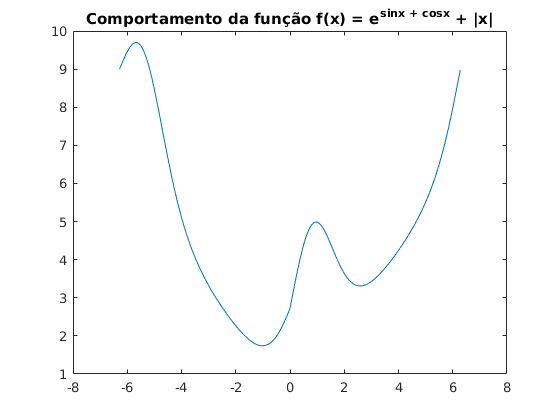
\includegraphics[width=1\linewidth]{image/sem_ruidos_y_fx}
		  \caption{\centering Mapeamento sem ruídos.} 
		  \label{fig:map1_s_ruido} 
		  
		\end{subfigure}%
		\begin{subfigure}{.5\textwidth}
		  \centering
		  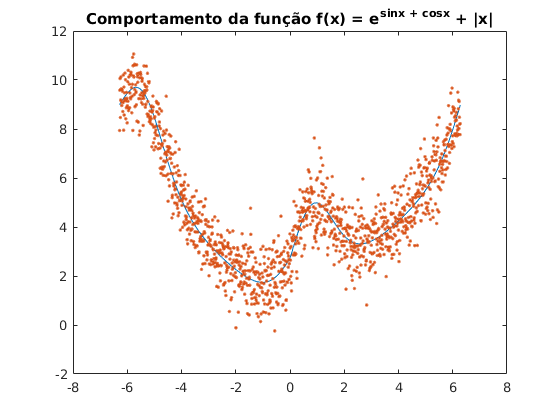
\includegraphics[width=1\linewidth]{image/com_ruidos_y_fx}
		  \caption{\centering Mapeamento com ruídos.}
		  \label{fig:map1_c_ruido} 
		\end{subfigure}
	
	
	\caption{Mapeamento da função \ref{eq:map1}.}
	\end{figure}
	
	\FloatBarrier
	
A simulação realizada no \textit{Eureqa}, primeiramente com os dados sem ruídos
e habilitando-se as funções-base exp(), sin(), cos(), abs() e as operações
básicas, forneceu os resultados contidos nas figuras
\ref{fig:map1_solucoes_s_ruido} e \ref{fig:map1_pareto_s_ruido}. A primeira
lista as soluções encontradas que mais se aproximaram dos dados amostrais.
Destaca-se que a primeira solução, cujo peso é 40, é justamente aquela que
utilizamos para produzir os dados. A segunda imagem ilustra o compromisso entre
acurácia (erro) e simplicidade (complexidade da solução). Observa-se que
inúmeras soluções apresentam erro praticamente nulo, porém existe apenas uma
cuja complexidade é mínima para este caso. Essa função trata-se da solução de
tamanho 40 que, como já foi dito, é igual à equação \ref{eq:map1}. A figura
\ref{fig:map1_best_s_ruido} apresenta um resumo da melhor solução encontrada.
Destaca-se que o erro podem ser considerados como nulos, visto que o maior erro
encontrado foi da ordem de \(10^{-14}\).

\FloatBarrier
			    
	\begin{figure}[h!]
	
	\centering
	
		\begin{subfigure}{.45\textwidth} 
		  \centering
		  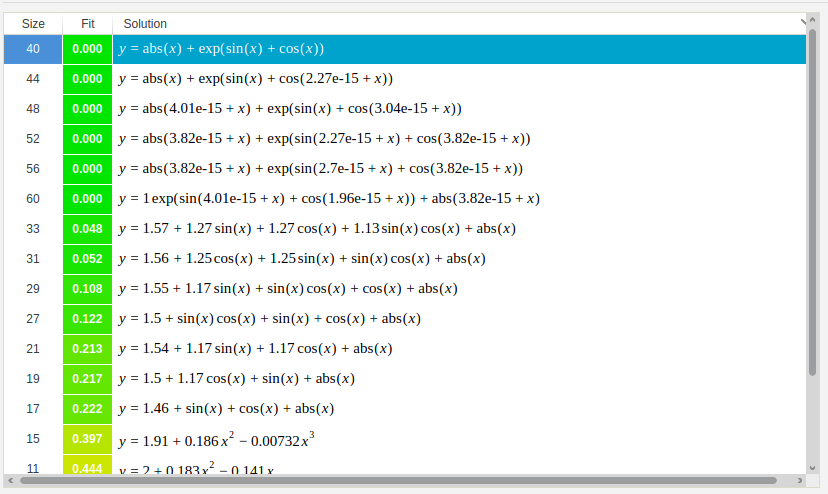
\includegraphics[width=1\linewidth]{image/solucoes_map1}
		  \caption{\centering Soluções encontradas pelo software.} 
		  \label{fig:map1_solucoes_s_ruido} 
		\end{subfigure}%
		\begin{subfigure}{.55\textwidth}
		  \centering
		  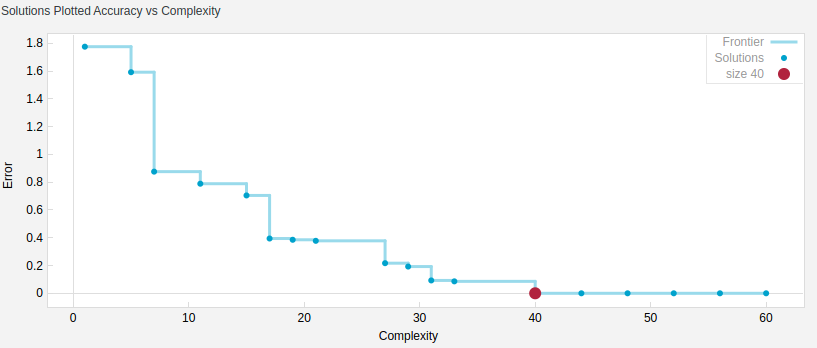
\includegraphics[width=1\linewidth]{image/pareto_map1}
		  \caption{\centering Compromisso acurácia \textit{x} simplicidade das
		  soluções.}
		  \label{fig:map1_pareto_s_ruido} 
		\end{subfigure}
	
		\begin{subfigure}{.65\textwidth}
		  \centering
		  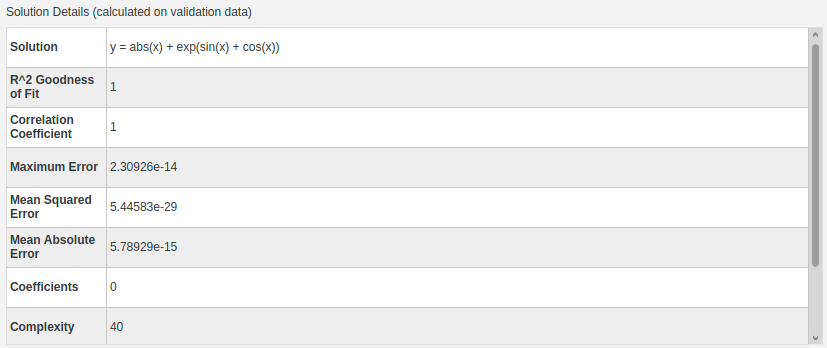
\includegraphics[width=1\linewidth]{image/best_solucao_map1}
		  \caption{\centering Resumo da melhor solução encontrada.}
		  \label{fig:map1_best_s_ruido} 
		\end{subfigure}
	
	\caption{Resultados para mapeamento da função \ref{eq:map1} sem ruídos.}
	\end{figure}
	
	\FloatBarrier

A simulação executada com os dados com ruído produziu o mapeamento representado
pela equação \ref{eq:map1_r}. A figura \ref{fig:comparaca_map1}  compara o mapeamento produzido
nesta fase com aquele utilizado para gerar os dados. Observa-se que ambos os
mapeamento estão muito próximos, porém há regiões em que as diferenças são
notáveis. Os resultados gerados pelo \textit{software} são, portanto, bastante
satisfatórios.

\begin{equation}
y = 1.61175 + 1.830094*\sin(0.792661 + x) +
0.55764*\sin(1.99325*x) + |x|
\label{eq:map1_r}
\end{equation}

\FloatBarrier
\begin{figure}[H]
		  \centering
		  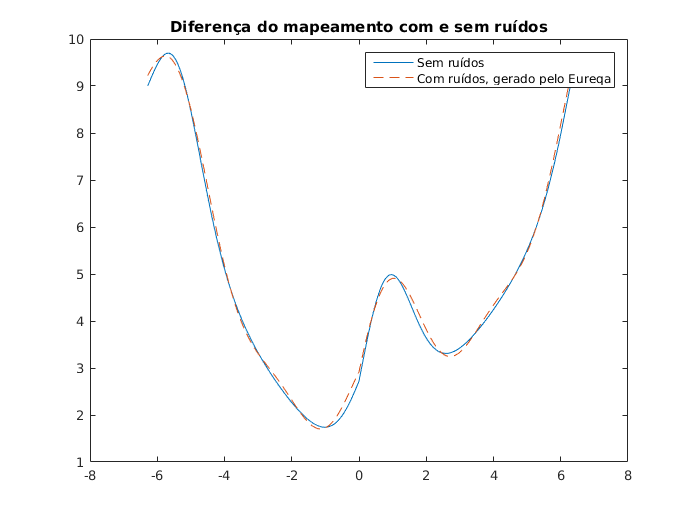
\includegraphics[width=0.65\linewidth]{image/comparacao_map1}
		  \caption{Comparação entre mapeamento com e sem ruídos.} 
		  \label{fig:comparaca_map1} 
		  
		\end{figure}
\FloatBarrier

As figuras \ref{fig:map1_solucoes_c_ruido}, \ref{fig:map1_pareto_c_ruido},
\ref{fig:map1_best_c_ruido}  e \ref{fig:map1_c_ruido} foram geradas pelo
\textit{Eureqa} e possuem informações sobre a solução encontrada. A primeira
é a lista de soluções encontradas pelo \textit{software}, a segunda mostra o
compromisso acurácia x complexidade (neste caso, a solução apresentada na
equação \ref{eq:map1_r} possui melhor compromisso, visto que seu erro é próximo
de 0 e sua complexidade, mínima), a terceira contem algumas informações sobre
a melhor solução (o erro quadrático médio neste caso é considerável,
contrariarmente ao caso sem ruído, e vale 0.625) e a última revela quais dados
foram usados para treinamento e validação, assim como o mapeamento encontrado.

\FloatBarrier
			    
	\begin{figure}[h!]
	
	\centering
	
		\begin{subfigure}{.45\textwidth} 
		  \centering
		  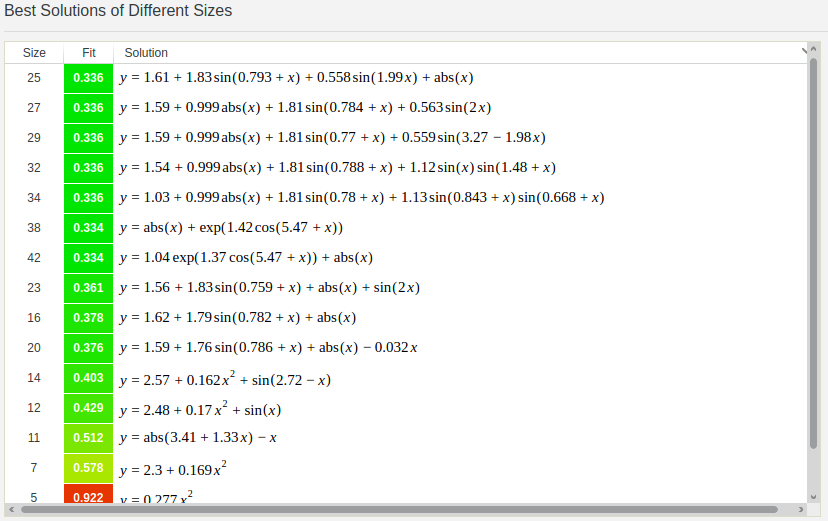
\includegraphics[width=1\linewidth]{image/best_solucao_map1_r}
		  \caption{\centering Soluções encontradas pelo software.} 
		  \label{fig:map1_solucoes_c_ruido} 
		\end{subfigure}%
		\begin{subfigure}{.55\textwidth}
		  \centering
		  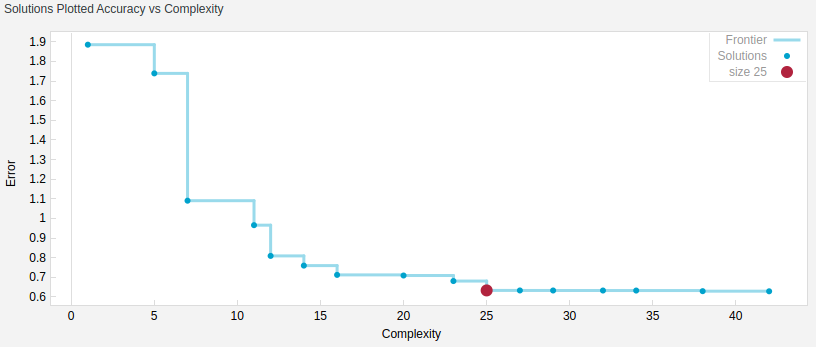
\includegraphics[width=1\linewidth]{image/pareto_map1_r}
		  \caption{\centering Compromisso acurácia \textit{x} simplicidade das
		  soluções.}
		  \label{fig:map1_pareto_c_ruido} 
		\end{subfigure}
	
		\begin{subfigure}{.5\textwidth}
		  \centering
		  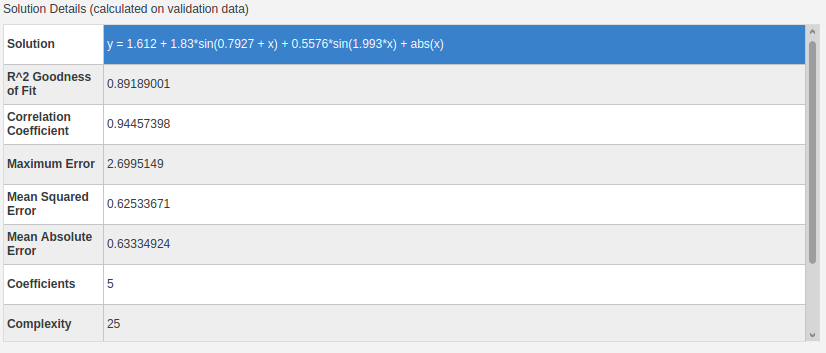
\includegraphics[width=1\linewidth]{image/best_solucao_map1_r_info}
		  \caption{\centering Resumo da melhor solução encontrada.}
		  \label{fig:map1_best_c_ruido} 
		\end{subfigure} %
		\begin{subfigure}{.45\textwidth}
		  \centering
		  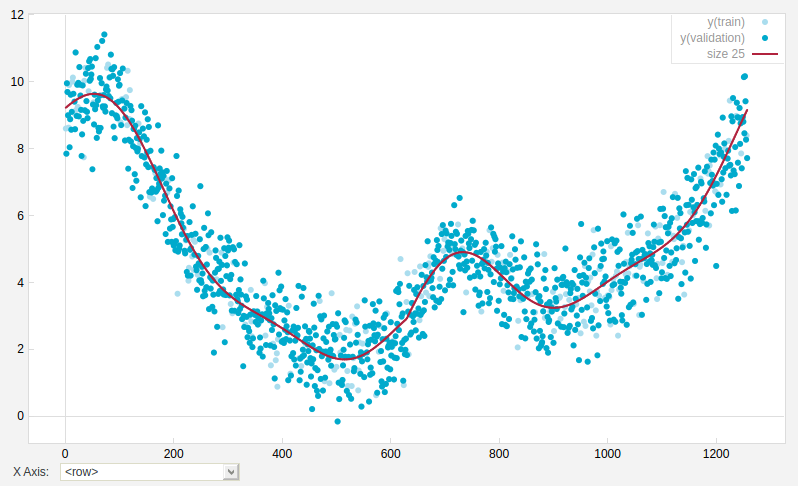
\includegraphics[width=1\linewidth]{image/solucoes_map1_r}
		  \caption{\centering Resumo do mapeamento encontrado e amostras usadas para
		  treinamento e validação.}
		  \label{fig:map1_c_ruido} 
		\end{subfigure}
	
	\caption{Resultados para mapeamento da função \ref{eq:map1} com ruídos.}
	\end{figure}
	
	\FloatBarrier

\subsection {Mapeamento y = f(x\textsubscript{1}, x\textsubscript{2},
x\textsubscript{3})}

A função escolhida para este caso está representada pela equação \ref{eq:map2},
sendo que \(x_1 \in [-3, 1]\), \(x_2 \in [1, 5]\) e \(x_3 \in [-4, 4]\). As duas
primeiras variáveis foram amostradas a cada 0.01 e a segunda, 0.02. Temos,
portanto, 401 amostras no total.

\begin{equation}
y = x_1*\log_{\pi}\left( \frac{x_2}{3}  \right) + \sqrt{2}*x_3 = 
x_1*\frac{\log_{10}\left( \frac{x_2}{3}  \right)}{\log_{10}(\pi)} + \sqrt{2}*x_3
\label{eq:map2}
\end{equation}

O mapeamento produzido pela simulação utilizando os dados sem ruídos
foi 

\begin{equation}
y =  0.959713 + 0.93436*x_3 + 0.873569*x_1*\log_{10}(x_2)
\label{eq:map2_s}
\end{equation}

O mapeamento produzido não corresponde ao utilizado para a geração dos dados,
porém os erros associados ao primeiro são praticamente nulos, isto é, o maior
erro é da ordem de \(10^{-15}\), conforme figura \ref{fig:map2_best_s_ruido}.
Isto indica que, para os os intervalos considerados para as variáveis, alguns
termos podem ser substituídos por outros sem perdas de precisão. Nota-se também,
pela figura \ref{fig:map2_solucoes_s_ruido}, que menos soluções foram encontradas em relação ao
item anterior. A imagem \ref{fig:map2_pareto_s_ruido} mostra o compromisso entre
erro e complexidade da melhor solução e é possível concluir, a partir desta
imagem, que realmente a solução de complexidade 15 supera as demais.

\FloatBarrier
			    
	\begin{figure}[h!]
	
	\centering
	
		\begin{subfigure}{.45\textwidth} 
		  \centering
		  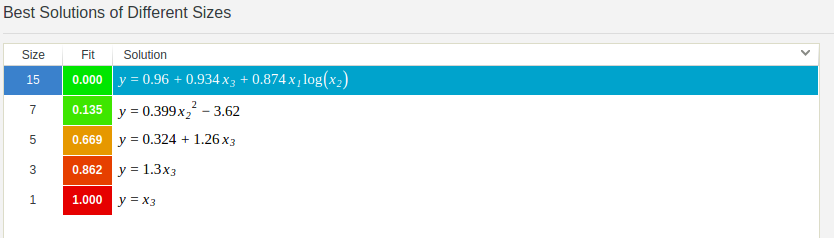
\includegraphics[width=1\linewidth]{image/solucoes_map2}
		  \caption{\centering Soluções encontradas pelo software.} 
		  \label{fig:map2_solucoes_s_ruido} 
		\end{subfigure}%
		\begin{subfigure}{.55\textwidth}
		  \centering
		  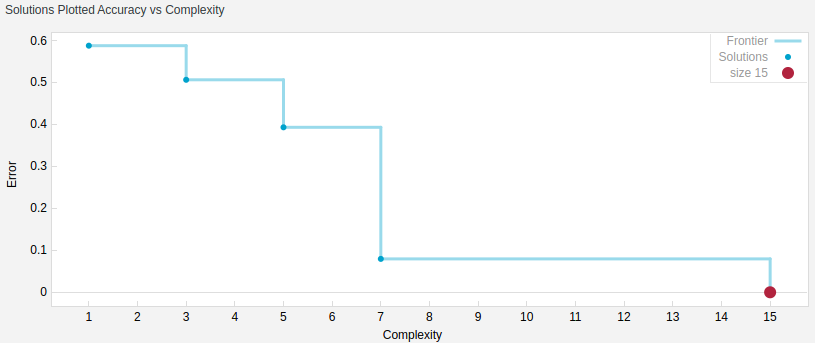
\includegraphics[width=1\linewidth]{image/pareto_map2}
		  \caption{\centering Compromisso acurácia \textit{x} simplicidade das
		  soluções.}
		  \label{fig:map2_pareto_s_ruido} 
		\end{subfigure}
	
		\begin{subfigure}{.65\textwidth}
		  \centering
		  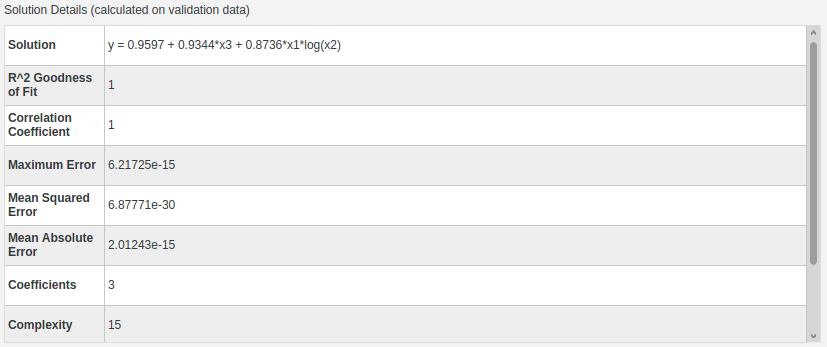
\includegraphics[width=1\linewidth]{image/best_solucao_map2_info}
		  \caption{\centering Resumo da melhor solução encontrada.}
		  \label{fig:map2_best_s_ruido} 
		\end{subfigure}
	
	\caption{Resultados para mapeamento da função \ref{eq:map2} sem ruídos.}
	\end{figure}
	
	\FloatBarrier

Enfim, a execução para os dados com ruídos gera o mapeamento 

\begin{equation}
y = 0.39025*x_2^2 - 3.555333
\label{eq:map2_r}
\end{equation}

Observa-se que \(y\) não depende de \(x_1\) e \(x_3\) neste caso. As figuras a
seguir foram geradas pelo \textit{software}. Destacam-se os seguintes fatos:

\begin{itemize}
  \item A figura \ref{fig:map2_pareto_c_ruido} mostra o compromisso entre erro e
  complexidade para as melhores soluções. Nota-se que, apesar de a solução não
  apresentar o menor erro, ela possui uma maior simplicidade comparada às
  demais. Sendo assim, ela é escolhida como a melhor solução atendendo aos
  critérios de acurácia e complexidade simultaneamente.
  \item Conforme figura \ref{fig:map2_best_c_ruido}, o erro quadrático médio é
  considerável e vale, aproximadamente, 0.70.
  \item A figura \ref{fig:map2_c_ruido} representa o mapeamento e as amostras
  utilizadas. Observa-se que este mapeamento aproxima-se relativamente bem aos
  dados.
\end{itemize}

\FloatBarrier
			    
	\begin{figure}[h!]
	
	\centering
	
		\begin{subfigure}{.45\textwidth} 
		  \centering
		  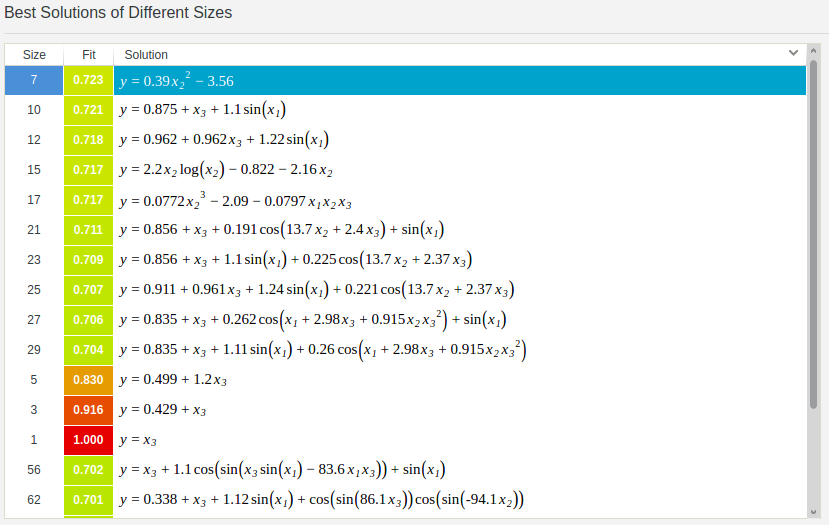
\includegraphics[width=1\linewidth]{image/solucoes_map2_r}
		  \caption{\centering Soluções encontradas pelo software.} 
		  \label{fig:map2_solucoes_c_ruido} 
		\end{subfigure}%
		\begin{subfigure}{.55\textwidth}
		  \centering
		  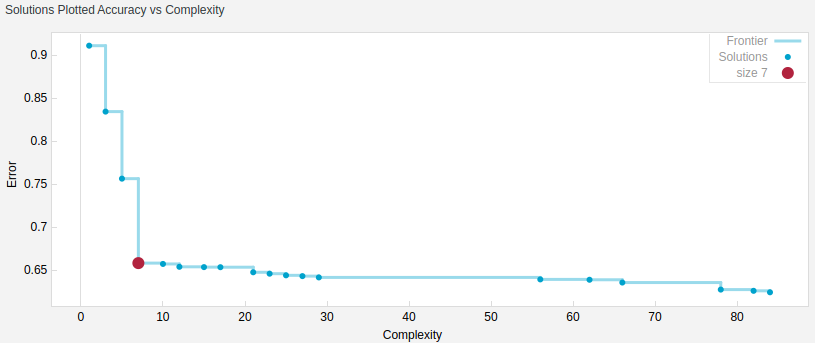
\includegraphics[width=1\linewidth]{image/pareto_map2_r}
		  \caption{\centering Compromisso acurácia \textit{x} simplicidade das
		  soluções.}
		  \label{fig:map2_pareto_c_ruido} 
		\end{subfigure}
	
		\begin{subfigure}{.5\textwidth}
		  \centering
		  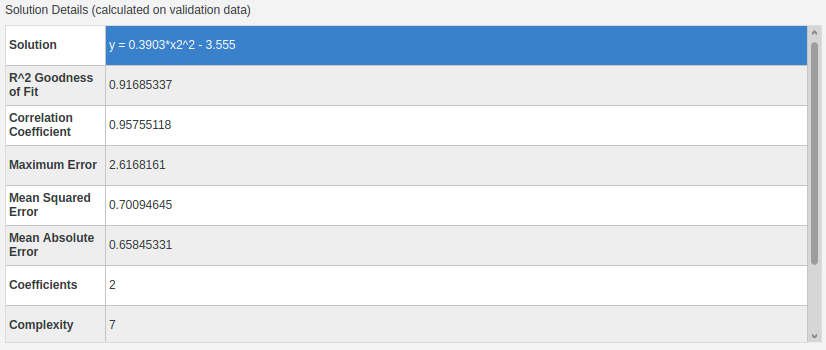
\includegraphics[width=1\linewidth]{image/best_solucao_map2_r_info}
		  \caption{\centering Resumo da melhor solução encontrada.}
		  \label{fig:map2_best_c_ruido} 
		\end{subfigure} %
		\begin{subfigure}{.45\textwidth}
		  \centering
		  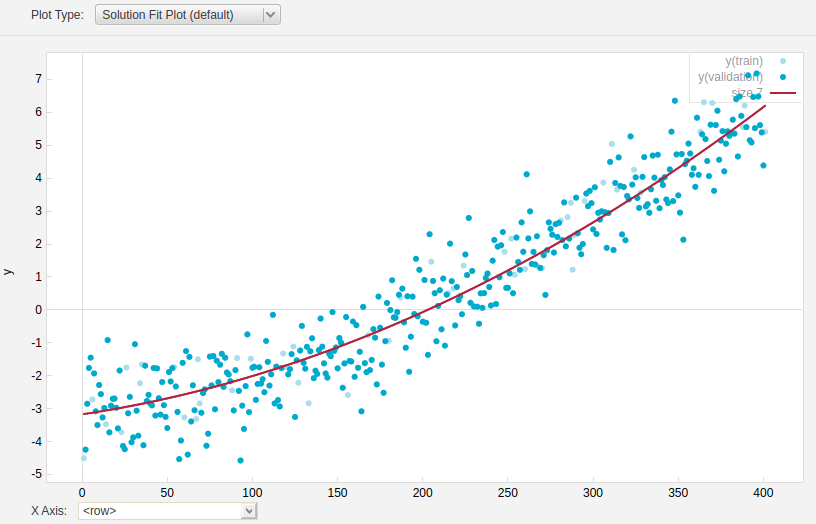
\includegraphics[width=1\linewidth]{image/best_solucao_map2_r}
		  \caption{\centering Resumo do mapeamento encontrado e amostras usadas para
		  treinamento e validação.}
		  \label{fig:map2_c_ruido} 
		\end{subfigure}
	
	\caption{Resultados para mapeamento da função \ref{eq:map2} com ruídos.}
	\end{figure}
	
	\FloatBarrier 


\section{Controle Nebuloso e Robótica Evolutiva}

\setcounter{subsection}{-1}
\subsection{Definição dos Consequentes }

O primeiro passo no controle do robô é a definição dos consequentes das regras
que serão levadas em conta. Considerando que o robô dispõe de 3 sensores
(\(d_1\), \(d_2\) e \(d_3\)) e que as funções de pertinência associadas às
medidas realizadas por eles estão representadas na seção 3 do enunciado, sugestões de consequentes estão
representadas na tabela \ref{tab:consequentes}, logo abaixo. As regras são da
forma \textbf{SE (\(d_1\) É x) E (\(d_2\) É y) E (\(d_3\) É z) ENTÃO
(\(\Delta \theta\) É w)}.

				\begin{table}[H]
					\centering
					\caption{\label{tab:consequentes} Regras que controlarão o robô.}
					\setlength\tabcolsep{4pt}
					\begin{minipage}{0.30\textwidth}
					    \centering
						\begin{tabular}{| c | c | c | c |} 
						\hline
						\(d_1\) & \(d_2\) & \(d_3\) & \(\Delta \theta\) \\ \hline
						P & MP & P & MN  \\ \hline
						P & MP & M & MN \\ \hline
						P & MP & G & MN \\ \hline
						P & PP & P & Z  \\ \hline
						P & PP & M & MN \\ \hline
						P & PP & G & MN \\ \hline
						P & PG & P & Z  \\ \hline
						P & PG & M & MN \\ \hline
						P & PG & G & MN \\ \hline
						P & MG & P & Z  \\ \hline
						P & MG & M & PN \\ \hline
						P & MG & G & MN \\ \hline
						\end{tabular}	
					\end{minipage}	      
					\begin{minipage}{0.30\textwidth}
					    \centering
						\begin{tabular}{| c | c | c | c |} 
						\hline
						\(d_1\) & \(d_2\) & \(d_3\) & \(\Delta \theta\) \\ \hline
						M & MP & P & PP \\ \hline
						M & MP & M & MP \\ \hline
						M & MP & G & MN \\ \hline
						M & PP & P & PP \\ \hline
						M & PP & M & Z  \\ \hline
						M & PP & G & PN \\ \hline
						M & PG & P & PP \\ \hline
						M & PG & M & Z  \\ \hline
						M & PG & G & PN \\ \hline
						M & MG & P & PP \\ \hline
						M & MG & M & Z  \\ \hline
						M & MG & G & PN \\ \hline
						\end{tabular}	
					\end{minipage}	
					\begin{minipage}{0.30\textwidth}
					    \centering
						\begin{tabular}{| c | c | c | c |} 
						\hline
						\(d_1\) & \(d_2\) & \(d_3\) & \(\Delta \theta\) \\ \hline
						G & MP & P & MP \\ \hline
						G & MP & M & MP \\ \hline
						G & MP & G & MP \\ \hline
						G & PP & P & MP \\ \hline
						G & PP & M & MP \\ \hline
						G & PP & G & MP  \\ \hline 	  	 
						G & PG & P & MP \\ \hline
						G & PG & M & PP \\ \hline
						G & PG & G & Z  \\ \hline
						G & MG & P & MP \\ \hline
						G & MG & M & PP \\ \hline
						G & MG & G & Z  \\ \hline
						\end{tabular}	
					\end{minipage}	      
			    \end{table}
	\FloatBarrier
	
	\subsection{Controlando o Robô}
	
	Uma vez definidas as regras que deverão ser seguidas, o próximo passo é então
	simular o comportamento do robô através do \textit{software} MATLAB. Para isso,
	5 funções foram escritas. A primeira, chamada \texttt{trap\_pertinencia},
	recebe 6 parâmetros, sendo eles a coordenada \(x\), as informações \(a\), \(b\), \(c\)
	e \(d\) referentes os trapézios que compõem as funções de pertinência e o valor
	a ser considerado caso \(x\) esteja fora do intervalo \(\left[a, d\right]\), e
	retorna o respectivo valor da função de pertinência. O programa
	\ref{lst:trap_pertinencia} abaixo possui a implementação da respectiva
	função.
	
	\lstinputlisting [language=Matlab, caption={ \texttt{trap\_pertinencia.m} -
	Avalia pertinência de um regra em função de \(x\).},
	label={lst:trap_pertinencia}] {image/trap_pertinencia.m}
	
	\vspace{12pt}
	
	A segunda função, chamada de \texttt{get\_D1\_D3\_Rule} e representada pelo
	programa \ref{lst:d1d3}, calcula a pertinência de cada um dos possíveis estados
	referentes aos sensores \(D_1\) e \(D_3\).	Essa função recebe como parâmetro a
	distância medida pelo sensor e retorna um vetor com três valores contendo a
	pertinência para os estados \textbf{P}, \textbf{M} e \textbf{G}. 
	
	\lstinputlisting [language=Matlab, caption={
	Avalia pertinência da regras de \(D_1\) e \(D_3\) em função das distâncias
	medidas.}, label={lst:d1d3}] {image/get_D1_D3_Rule.m}

	\vspace{12pt}
	
	A função \texttt{get\_D2\_Rule} realiza o mesmo que o descrito anteriormente,
	mas agora com o sensor \(D_2\). A implementação desta função pode ser
	encontrada logo abaixo.
	
	\lstinputlisting [language=Matlab, caption={
	Avalia pertinência da regras de \(D_2\) em função das distâncias
	medidas.}, label={lst:d2}] {image/get_D2_Rule.m} 
	
	\vspace{12pt}
	
	A quarta função, \texttt{get\_Angle\_Rule}, implementa as regras descritas na
	tabela \ref{tab:consequentes}. Por ser extensa, a sua implementação foi
	colocada na seção \textbf{Anexos} ao fim deste documento no programa
	\ref{lst:angle_rule}. Em poucas palavras, esta função testa se cada uma das
	regras está ativa e, caso uma determinada regra esteja, atribui a ela o menor
	valor dentre as pertinências dos estados que a compõem. Por exemplo, se \(D_1\)
	é \textbf{P} com 50\%, \(D_2\) é \textbf{MG} com 100\% e \(D_3\) é \textbf{M}
	com 33\%, então \(\Delta \theta\) é \textbf{PN} com 33\%.
	
	\vspace{12pt}
	
	A quinta função, \texttt{get\_Angle}, é responsável pelo processo de
	\textit{defuzzyficação} e está representada pelo programa \ref{lst:angle}. Ela
	utiliza o método de centro de massa para determinar \(\Delta \theta\) que
	melhor convém dadas as regras ativas.
	
	\lstinputlisting [language=Matlab, caption={
	Avalia pertinência da regras de \(D_2\) em função das distâncias
	medidas.}, label={lst:angle}] {image/get_Angle.m}
	
	\vspace{12pt}
	
	Enfim, a sexta função, \texttt{robot\_control}, realiza o controle do robô
	conforme regras especificadas acima. Sua implementação está representada pelo
	programa \ref{lst:control}.
	
	\lstinputlisting [language=Matlab, caption={  
	Automatiza controle do robô.}, label={lst:control}] {image/robot_control.m}  
	
	\subsection {Resultados}
	
	A fim de testar o controlador implementado na seção anterior, dois mapas foram
	criados. Os resultados das execuções estão representados na figuras
	\ref{fig:test_fuzzy_1} e \ref{fig:test_fuzzy_2}, em que a trajetória está
	representada em preto, a parede em cinza claro, os pontos de destino em cinza
	escuro e as posições livres, em branco. Para ambos, a direção inicial do robô é
	\(\frac{\pi}{2}\), as coordenadas iniciais são \((3,3)\) e a velocidade é \(v =
	1 \) \textit{pixel/iteração}. Verifica-se que o controle é bem-sucedido, sendo
	que o robô é capaz de realizar as curvas presentes nos mapas. É importante
	comentar que os cantos \textit{suavizados} possuem uma grande importância para o
	bom resultado, uma vez que o controle nas áreas de ``ponta'' não é tão eficiente
	visto que, quando o controlador verifica a proximidade a uma parede, ele pode
	não saber para que lado virar.
		
	\FloatBarrier
			    
	\begin{figure}[h!]
	
	\centering
	
		\begin{subfigure}{.5\textwidth}
		  \centering
		  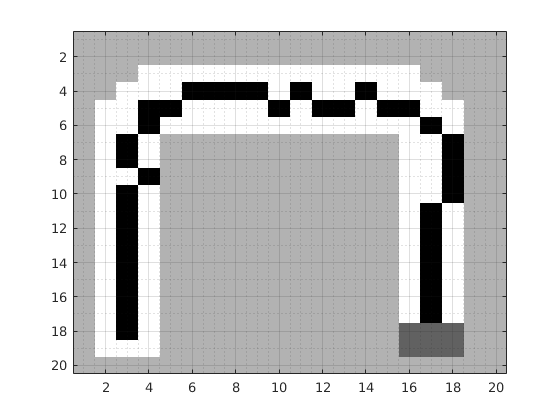
\includegraphics[width=1\linewidth]{image/test1}
		  \caption{\centering Controle do robô no mapa 1.}
		  \label{fig:test_fuzzy_1}
		  
		\end{subfigure}%
		\begin{subfigure}{.5\textwidth}
		  \centering
		  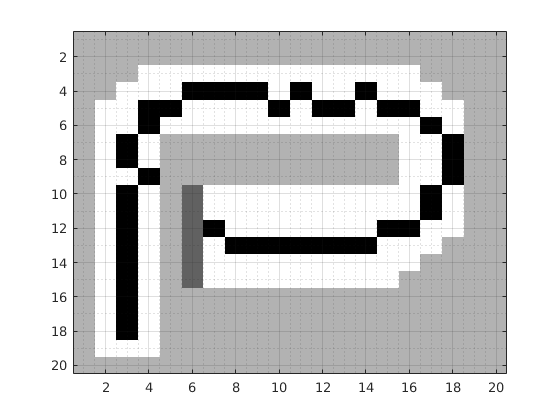
\includegraphics[width=1\linewidth]{image/test2}
		  \caption{\centering Controle do robô no mapa 2.}
		  \label{fig:test_fuzzy_2} 
		\end{subfigure}
	
	
	\caption{Resultados para o controle nebuloso do robô
	para dois mapas distintos.}
	\end{figure} 
	
	\FloatBarrier
		
	O \textit{script} utilizado nos testes pode ser encontrado no programa
	\ref{lst:test_fuzzy}.
	
	\lstinputlisting [language=Matlab, caption={  
	\textit{Script} de teste..}, label={lst:test_fuzzy}]
	{image/test_robot_control.m}

	\subsection {Controle via Rede Neural MLP}
	
	A adaptação do controle do robô via redes neurais exigiu algumas modificações
	nos programas fornecidos anteriormente nesta seção e também no algoritmo de
	evolução fornecido pelo professor, que foi utilizado na seção \ref{sec:pid}.
	Foram utilizados, neste caso, \(N = 10\) para a camada intermediária, 100
	gerações e 100 indivíduos na população.
	
	\vspace{12pt}
	
	Para o algoritmo evolutivo, foram alteradas a função de \textit{fitness}, a
	estrutura do cromossomo e as taxas de mutação e \textit{crossover}, conforme
	explicado a seguir.
	
	\begin{itemize}
	  \item A função de \textit{fitness} utilizada foi
	  \(f_{fitness}=\frac{1}{n_{colisao} + 1}\). Logo, soluções que obtiverem
	  muitas colisões serão piores, isto é, terão um \textit{fitness} menor. A
	  linha adicionada ao código foi, portanto:
	  
\begin{lstlisting}[language=Matlab, style=nonumbers]
fitness(i,1) = 1/(colision_i + 1);
\end{lstlisting}
	
	  \item  Anteriormente, tínhamos apenas 3 parâmetros a evoluir, sendo eles
	  \(k_d\), \(k_p\) e \(k_i\). Neste caso, o número de parâmetros depende do
	  número de neurônios na camada intermediária. Sejam \(N\) neurônios nesta
	  camada, cada um deles terá 4 pesos, sendo um deles para a entrada constante e
	  o restante para as distâncias dos sensores. Há ainda mais \(N + 1\) pesos a
	  serem ajustáveis, correpondentes à soma dos resultados de cada neurônio. A
	  estrutura utilizada foi, portanto:
	  
\begin{lstlisting}[language=Matlab, style=nonumbers]
% Numero de entradas: d1, d2, d3 e termo constante
E = 3 + 1;
pop = randn(tam_pop, E * n_neurons + n_neurons + 1);
\end{lstlisting}	  
	
	  Utilizou-se também uma distribuição normal de média 0 e variância 1 para os
	  pesos iniciais da rede neural.
	  
	  \item A fim de maximizar a diversidade na rede, utilizou-se taxas de mutação
	  \(p_m = 0.8\) e \textit{crossover} \(p_c = 0.9\).

	\end{itemize}
	
	O controle do robô, realizado pela \texttt{robot\_control\_mlp}, também foi
	alterado. A linhas referentes ao controle nebuloso (linhas 75 a 86 do programa
	\ref{lst:control}) foram retiradas e substituídas pelo trecho de código abaixo.
	
\begin{lstlisting}[language=Matlab, caption={Trecho de código do controle do
robô feito via rede MLP.}, label={lst:control_mlp}] 
% Constroi vetor das entradas de cada neuronio
mlp_input = [distance_d1 distance_d2 distance_d3 1];

% middle_layer_output contera as saidas de cada neuronio da camanda
% intermediaria
middle_layer_output = zeros (1, n_neurons);

% Calcula a saida de cada neuronio. mlp_weights contem todos os pesos
% sinapticos da rede 
for n = 1 : n_neurons
    
    middle_layer_output (1, n) = ...
        tanh(mlp_input * mlp_weights (1 + (n - 1)* 4 : 4 + (n - 1)* 4)');
    
end

% a entrada da ultima camada eh a saida da camada intermediaria e uma
% termo constante.
last_layer_input = [middle_layer_output 1];

% Calcula o desvio na direcao do robo. Seleciona ultimos n_neurons + 1 pesos
% sinapticos. 
d_angle = ...
 last_layer_input * mlp_weights (1 + 4 * n_neurons : 1 + 4 * n_neurons + n_neurons)';

robot_direction = robot_direction + d_angle;

teste (round(m_length + 1 - y_robot), round(x_robot)) = 'r';

% Calcula nova posicao.
x_robot = x_robot + speed*cos(robot_direction);
y_robot = y_robot + speed*sin(robot_direction);

% Verifica se a nova posicao esta dentro do mapa.
if (round(x_robot) > length(labyrinth_matrix (1,:))) ...
        || (round(x_robot) < 1) ...
        || (round(m_length + 1 - y_robot) < 1) ...
        || (round(m_length + 1 - y_robot) > m_length)
    
    % Penalisa movimentos que levam o robo fora do mapa.
    colisions = colisions + 1000;
    
% Detecta colisao.
elseif (labyrinth_matrix (round(m_length + 1 - y_robot), round(x_robot)) == '#')
    
    % Aumenta contador de colisoes.
    colisions = colisions + 1;
end
\end{lstlisting}
	
O mapa da figura \ref{fig:test_fuzzy_2} foi utilizado no treinamento da rede
neural, visto que apresenta situações mais desafiadoras que o mapa da figura
\ref{fig:test_fuzzy_1}. Sendo assim, acredita-se que se o programa for
bem-sucedido em calcular os pesos sinápticos para o mapa mais complexo, então,
os mesmos pesos serão adequados para mapas mais simples. As figuras
\ref{fig:mlp_2} e \ref{fig:mlp_1} contém resultados para um dos vetores de
pesos sinápticos encontrado pelo algoritmo evolutivo em que essa afirmação é
comprovada.

\FloatBarrier
			    
	\begin{figure}[h!]
	
	\centering
	
		\begin{subfigure}{.5\textwidth}
		  \centering
		  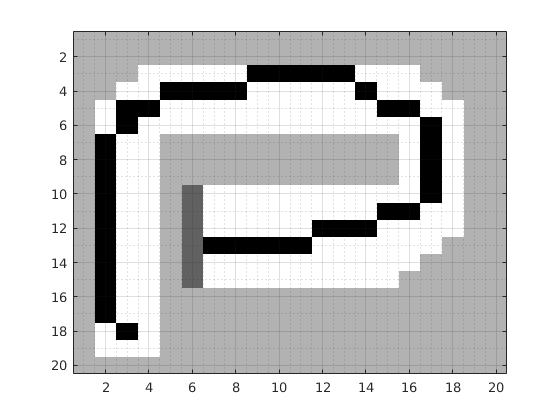
\includegraphics[width=1\linewidth]{mlp_robot/mlp_2}
		  \caption{\centering Controle do robô via MLP no mapa 2.}
		  \label{fig:mlp_2}
		  
		\end{subfigure}%
		\begin{subfigure}{.5\textwidth}
		  \centering
		  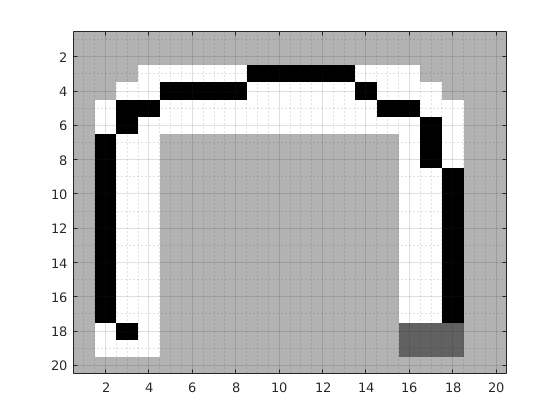
\includegraphics[width=1\linewidth]{mlp_robot/mlp_1}
		  \caption{\centering Controle do robô via MLP no mapa 1}
		  \label{fig:mlp_1} 
		\end{subfigure}
	
	
	\caption{Resultados para o controle do robô via MLP
	para dois mapas distintos.}
	\end{figure} 
	
	\FloatBarrier
	
	A figura \ref{fig:fitness_mlp} representa a evolução do \textit{fitness} ao
	decorrer da execução do algoritmo evolutivo. Verifica-se que, apesar da melhor
	solução ser encontrada nas primeiras gerações, o \textit{fitness} médio é muito
	pequeno em todas as gerações. Esse fato pode ser explicado pelos valores das
	taxas de mutação e \textit{crossover}, responsáveis por manter uma grande
	diversidade na população. Dessa forma, sempre serão adicionados à população
	indivíduos ruins, isto é, que produzem baixos \textit{fitness}.
	
	\FloatBarrier
	
	\begin{figure}[h]
    \centering
    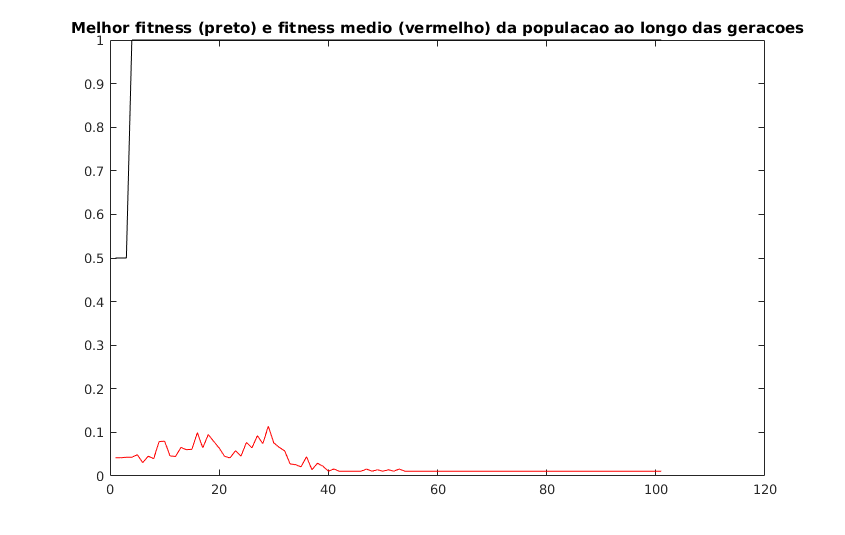
\includegraphics[scale=0.65]{mlp_robot/fitness}
    \caption{\label{fig:fitness_mlp}Evolução do \textit{fitness} médio e
    melhor.}
	\end{figure}  
	
	\FloatBarrier
	
	As figuras \ref{fig:mlp_2_1} e \ref{fig:mlp_2_2} foram obtidas pelo
	treinamento da rede neural no mapa da figura \ref{fig:test_fuzzy_1}.  
	
	\FloatBarrier
			    
	\begin{figure}[h!]
	
	\centering
	
		\begin{subfigure}{.5\textwidth}
		  \centering
		  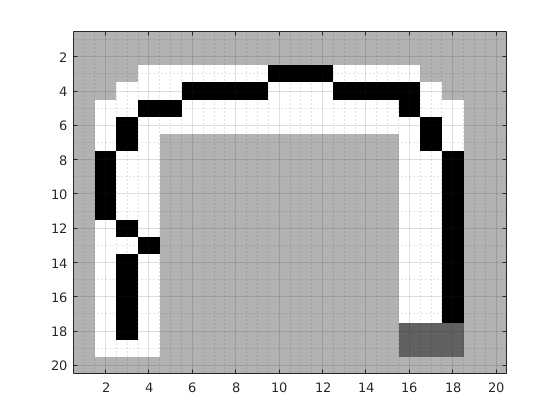
\includegraphics[width=1\linewidth]{mlp_robot/mlp_1_2}
		  \caption{\centering Controle do robô via MLP no mapa 1.}
		  \label{fig:mlp_2_1}
		  
		\end{subfigure}%
		\begin{subfigure}{.5\textwidth}
		  \centering
		  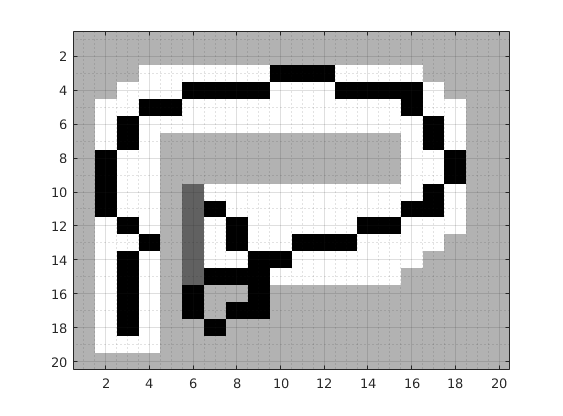
\includegraphics[width=1\linewidth]{mlp_robot/mlp_2_2}
		  \caption{\centering Controle do robô via MLP no mapa 2.}
		  \label{fig:mlp_2_2} 
		\end{subfigure}
	
	
	\caption{Resultados para o controle do robô via MLP
	para dois mapas distintos.}
	\end{figure} 
	
	\FloatBarrier
	
Verifica-se que a solução encontrada para o primeiro mapa, que é mais simples,
controla corretamente o robô. Entretanto, se o mesmo controle fosse utilizado
para o mapa 2, então o robô colidiria com a parede, conforme mostrado na figura
\ref{fig:mlp_2_2}. Isso é explicado pelo fato de que o mapa exige um controle
mais complexo que o primeiro.


\section{Conclusões}

Este exercício de fixação de conceitos mostrou todo o poder e abrangência das
técnicas de inteligência artificial, visto que diversos problemas de áreas
completamente distintas foram abordados e resolvidos. A primeira aplicação
consistiu na determinação dos parâmetros \(k_i\), \(k_d\) e \(k_p\) de um
controlador através de um algoritmo evolutivo. A determinação desses parâmetros
é complexa e exige um amplo conhecimento dos conceitos de controle e automação.
Sendo assim, o interesse da utilização de um algoritmo de IA é justamente propor
um método que possa contornar esse elevado grau de complexidade sem conhecer
intrinsecamente o problema, ainda que a solução encontrada não seja a ótima.
Destaca-se, entretanto, que as soluções encontradas foram muito satisfatórias
para os critérios selecionados, isto é, tempo de resposta e margem de fase.

\vspace{12pt}

Para a segunda aplicação, utilizamos o \textit{software} Eureqa para produzir
mapeamentos a partir de dados. Observou-se que, mesmo para dados contendo ruído,
o programa é capaz de produzir aproximações muito consistentes. Foi possível
igualmente manipular a ideia de equilíbrio de Pareto, à medida que várias
situações eram apresentadas com diversos graus de complexidade e precisão.

\vspace{12pt}

A terceira aplicação envolveu os conceitos de controle nebuloso e redes neurais
MLP. O controle do robô foi realizado por ambos os modelos. Foi possível
visualizar, portanto, que, apesar desses métodos serem baseados em princípios
completamente distintos, ambos conseguem resolver o problema. Uma das
características mais importantes dos algoritmos de inteligência artifial é
justamente a sua generalidade em resolver problemas de diferentes áreas.

\vspace{12pt}

Enfim, para os quarto e quintos exercícios, abordou-se o problema de
recomendação de notas para os usuários. Para isso, usamos a base
\textit{MovieLens} que contém uma grande quantidade de \textit{ratings}. O
primeiro método explorado foi o \textit{k-NN}, que não leva em consideração os
atributos de usuários e filmes na sua predição. Este algoritmo só considera os
\(k\) vizinhos mais próximos de um usuário determinado. Exploramos também o
algoritmo SCOAL, mais robusto que o primeiro, que utiliza os atributos
discutidos anteriormente e divide a matriz de dados em \textit{co-clusters},
para os quais modelos preditivos são calculados.


\section{Referências}

\begin{itemize}
  \item \url{https://en.wikipedia.org/wiki/Precision_and_recall}. \\
  		Acessado às 20:29 17/11/2015

  \item L. Candillier, K. Jack, F. Fessant, F. Meyer, ``State-of-the-Art
Recommender Systems''.

  \item   M. Deodhar, J. Ghosh, ``SCOAL: A Framework for Simultaneous
Co-Clustering and Learning from Complex Data''.

\end{itemize}

\newpage
\section{Anexos}
\subsection{Programas}

\lstinputlisting [language=Matlab, caption={
Função que implementa regras nebulosas.},
label={lst:angle_rule} ]{../src/fuzzy/get_Angle_Rule.m}
 

    
\end{document}
